\chapter{Related Work}

\label{ch:related_work}

%
%
%
%
%
\section{Autoencoders}

An autoencoder is a neural network that learns a compression algorithm for its input data in an unsupervised manner \cite{Liou2008}. This is achieved by placing constraints on a hidden layer, called the latent space, and setting the target values to the input values, effectively learning the identity function. Since the network is trying to reconstruct the original input from the constrained latent space, over time the latent space corresponds to a meaningful compression of the network's input.

\begin{figure}[h!]
\centering
\captionsetup{justification=centering}
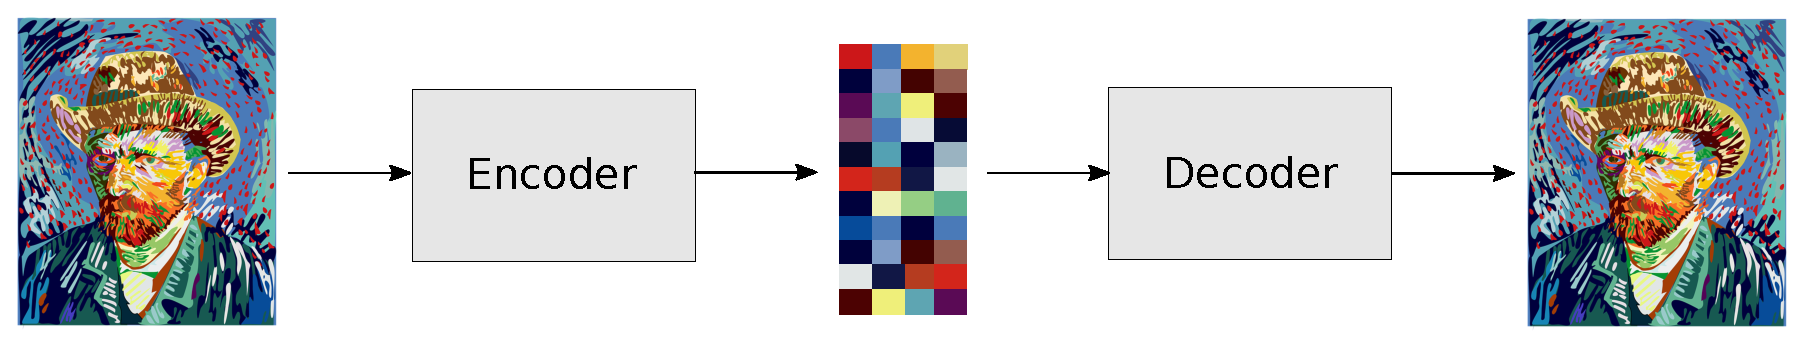
\includegraphics[scale=0.53]{background/autoencoder_black_box_architecture.eps}
\caption{A black-box description of an autoencoder. The autoencoder learns the identity function, and in turn, the encoder and decoder learn suitable encoding and decoding algorithms respectively.}
\label{fig:autoencoder_black_box_architecture}
\end{figure}

As before, we will use the MNIST data set to compare architectures. Unless specified in the example, the Adam optimiser is used with a learning rate of $1e-4$, the batch size is 1 and the loss function is binary cross-entropy. Intermediate layers use the ReLU activation function, while the final layer uses sigmoid.

\subsection{Fully-Connected Autoencoders}

In dense feed-forward neural networks we may place a constraint on the latent space by reducing the number of neurons, as shown in Figure \ref{fig:autoencoder_architecture}. Images must be flattened into vectors to be fed as input. Consequently, any spatial information is destroyed in dense feed-forward neural networks.

\begin{figure}[h!]
\centering
\captionsetup{justification=centering}
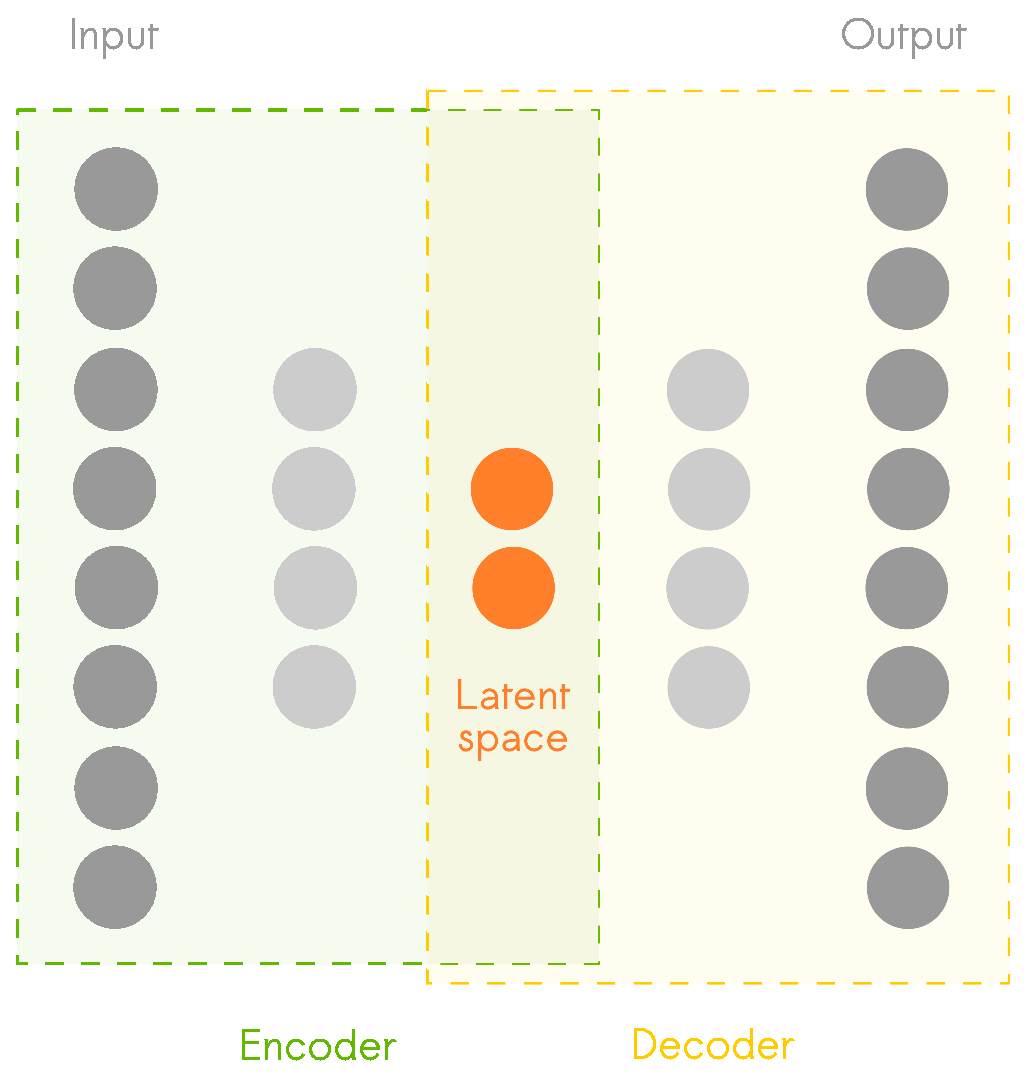
\includegraphics[scale=0.5]{background/autoencoder_architecture.eps}
\caption{An example architecture of a fully-connected autoencoder. The latent space is constrained by having fewer neurons than the input and output layers.}
\label{fig:autoencoder_architecture}
\end{figure}

An example architecture is given in Table \ref{tab:fully_connected_autoencoder_architecture}, which was trained on MNIST. Despite the latent space being $\sim4\%$ of the size of the input space, the network is capable of producing realistic reconstructions. For verification, a collection of samples from the dataset and their corresponding reconstructions are shown in Figure \ref{fig:fully_connected_autoencoder_mnist}.

\begin{table}[h!]
\centering
\captionsetup{justification=centering}
\begin{tabular}{@{}ll@{}}
\toprule
\textbf{Layer Type} & \textbf{Output Shape} \\ \midrule
InputLayer & (1, 28, 28) \\
Flatten & (784,) \\
Dense & (32,) \\
Dense & (784,) \\
Reshape & (1, 28, 28) \\ \bottomrule
\end{tabular}
\caption{A simple fully-connected autoencoder with one hidden layer. After 15 epochs, the validation score was recorded to be $71.94$.}
\label{tab:fully_connected_autoencoder_architecture}
\end{table}

\begin{figure}[H]
\centering
\captionsetup{justification=centering}
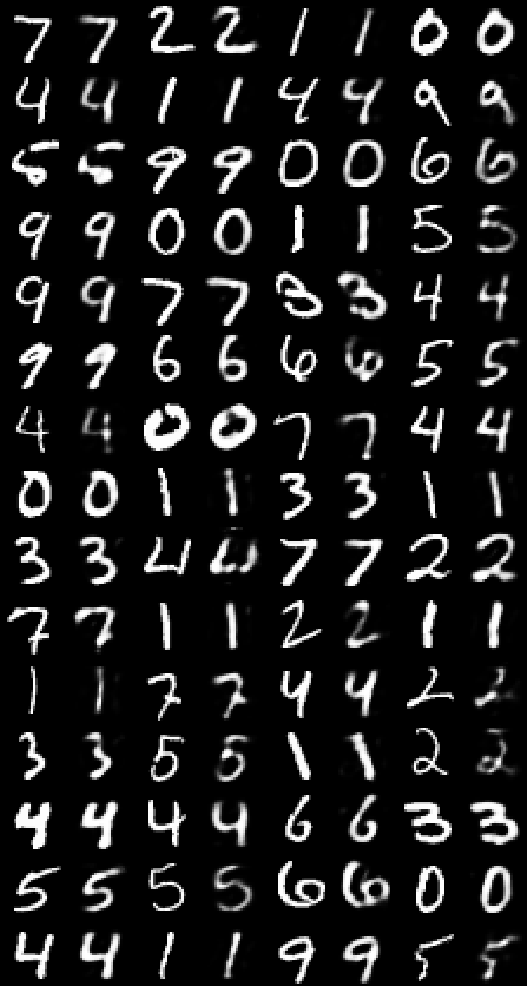
\includegraphics[scale=0.95]{background/fully_connected_autoencoder_mnist.png}
\caption{A collection of images from the MNIST data set and their respective reconstructions using the fully-connected autoencoder specified in Table \ref{tab:fully_connected_autoencoder_architecture}. The original MNIST images are in odd columns, and their reconstructions to their immediate right.}
\label{fig:fully_connected_autoencoder_mnist}
\end{figure}

\subsection{Fully-Convolutional Autoencoders}

In fully-convolutional feed-forward neural networks, we may place a constraint on the latent space by reducing the number and/or size of the filters, as shown in Figure \ref{fig:convolutional_autoencoder_architecture}. To compare the fully-convolutional autoencoder to the fully-connected, we'll train the architecture in Table \ref{tab:convolutional_autoencoder_architecture} on MNIST. As before, we'll compare the reconstructions to the originals, which can be found in Figure \ref{fig:convolutional_autoencoder_mnist}.\\

\begin{figure}[h!]
\centering
\captionsetup{justification=centering}
\includegraphics[scale=0.6]{background/convolutional_autoencoder_architecture.eps}
\caption{An example architecture of a fully-convolutional autoencoder. The latent space is constrained by reducing the number and/or size of the filters.}
\label{fig:convolutional_autoencoder_architecture}
\end{figure}

\vspace{8mm}

\begin{table}[h!]
\centering
\captionsetup{justification=centering}
\begin{tabular}{@{}ll@{}}
\toprule
\textbf{Layer Type} & \textbf{Output Shape} \\ \midrule
InputLayer & (1, 28, 28) \\
Conv2D & (32, 28, 28) \\
MaxPooling2D & (32, 14, 14) \\
Conv2D & (4, 14, 14) \\
MaxPooling2D & (4, 7, 7) \\
UpSampling2D & (4, 14, 14) \\
Conv2DTranspose & (32, 14, 14) \\
UpSampling2D & (32, 28, 28) \\
Conv2DTranspose & (1, 28, 28) \\ \bottomrule
\end{tabular}
\caption{A simple fully-convolutional autoencoder with 2D convolutions and max pooling, plus the corresponding deconvolutional layers. After 15 epochs, the validation score was recorded to be $64.89$.}
\label{tab:convolutional_autoencoder_architecture}
\end{table}

Convolutional layers have been shown to be effective in tasks with images as input \cite{Krizhevsky2012, Zeiler2014, Szegedy2015}. This is because spatial information is preserved in convolutional layers, and the number of trainable parameters is far less in a convolutional layer than it is in a fully connected layer. Convolutional layers will be used from here on as we'll be using images as input.

\newpage
\begin{figure}[H]
\centering
\captionsetup{justification=centering}
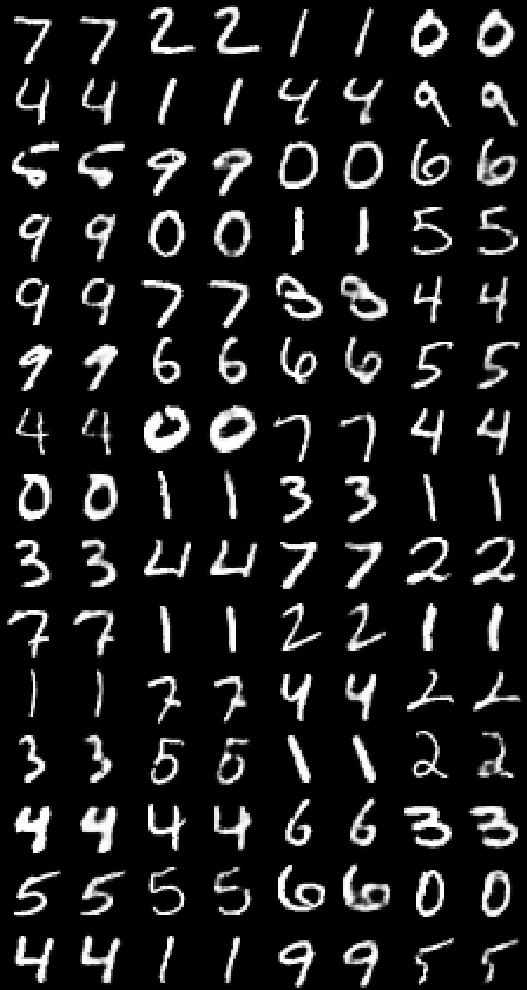
\includegraphics[scale=0.95]{background/fully_convolutional_autoencoder_mnist.png}
\caption{A collection of images from the MNIST data set and their respective reconstructions using the fully-convolutional autoencoder specified in Table \ref{tab:convolutional_autoencoder_architecture}. The original MNIST images are in odd columns, and their reconstructions to their immediate right.}
\label{fig:convolutional_autoencoder_mnist}
\end{figure}


%
%
%
%
%
\section{Variational Autoencoders}
\label{sec:variational_autoencoders}
\cite{Kingma2014}

The variational autoencoder is central to this project, and we'll therefore dedicate a considerable amount of time exploring it. First we'll precisely define the problems the variational autoencoder solves, after which we may develop its loss function and detail its implementation. This section will conclude by developing an intution of the theory covered by way of examples.

\subsection{A Probabilistic Perspective}
We'll begin by making necessary definitions and describe the input data as samples from a generative process.. This sets the context to detail the problems the variational autoencoder solves.

Let $X = \{\vec{x}^{(i)}\}_{i=1}^{N}$ be the data set of $N$ independent and identically distributed samples of the variable $\vec{x}$. ($X$ may be a data set of images, for instance). Let us assume that these samples are generated by a random process with parameters $\vec{\theta^*}$ involving an unobserved latent variable $\vec{z}$ in the following way:\\

\begin{algorithm}
  \caption{Generate data set $X$}
  \begin{algorithmic}[1]
  \For{$i = 1 \to N$}
      \State $\vec{z}^{(i)} \sim p_{\vec{\theta}^*}(\vec{z})$ \quad\quad\quad\quad\quad\quad\quad\quad\quad\quad // Sample from true prior
      \State $\vec{x}^{(i)} \sim p_{\vec{\theta}^*}(\vec{x} | \vec{z}^{(i)})$ \quad\quad\quad\quad\quad\quad\quad\enspace\enspace\thinspace // Sample from true conditional
      \State Append $\vec{x}^{(i)}$ to $X$
  \EndFor
  \end{algorithmic}
  \label{alg:generate_data_set_x}
\end{algorithm}

We only observe the data set $X$ in this process. The parameters $\vec{\theta}^*$ and latent variables $Z = \{ \vec{z}^{(i)} \}_{i=1}^{N}$ are unknown to us. Let us assume that the prior $p_{\vec{\theta^*}}(\vec{z})$ and conditional $p_{\vec{\theta^*}}(\vec{x}|\vec{z})$ are parameterised by the distributions $p_{\vec{\theta}}(\vec{z})$ and $p_{\vec{\theta}}(\vec{x}|\vec{z})$ respectively. In this context, the variational autoencoder provides \cite{Kingma2014}:

\begin{enumerate}
\item ML or MAP estimation for the parameters $\vec{\theta}$
\item An approximation of the latent variable $\vec{z}^{(i)}$ given $\vec{x}^{(i)}$ and set of parameters $\vec{\theta}$
\item Approximate marginal inference of the variable $\vec{x}$
\end{enumerate}

\subsection{Overcoming the Intractable Posterior}
The variational autoencoder solves the problems above by approximate inference of the latent variable $\vec{z}$. Exact inference is not possible, and to see this we may use Bayes' theorem to find an expression for the posterior:
\begin{align}
p_{\vec{\theta}}(\vec{z}|\vec{x}) = \frac{p_{\vec{\theta}}(\vec{x}|\vec{z})p_{\vec{\theta}}(\vec{z})}{p_{\vec{\theta}}(\vec{x})}
\end{align}
The marginal likelihood
\begin{align}
p_{\vec{\theta}}(\vec{x}) = \int p_{\vec{\theta}}(\vec{z})p_{\vec{\theta}}(\vec{x}|\vec{z})d\vec{z}
\end{align}
involves an exponential-time integral over every combination of the latent variable $\vec{z}$, and is therefore computationally intractable \cite{Kingma2014}. Instead, we define an approximation $q_{\vec{\phi}}(\vec{z}|\vec{x})$ to the intractable posterior. Since $q_{\vec{\phi}}(\vec{z}|\vec{x})$ gives a distribution over the possible latent variables $\vec{z}$ that generated the given data point $\vec{x}$, it is known as the probabilistic decoder. By the same reasoning, $p_{\vec{\theta}}(\vec{x}|\vec{z})$ is known as the probabilistic decoder.

\subsection{Finding a Suitable Loss Function: the ELBO}
The variational autoencoers's ability to learn the generative parameters $\vec{\theta}^*$ relies on how closley $q_{\vec{\phi}}(\vec{z}|\vec{x})$ approximates $p_{\vec{\theta}}(\vec{z}|\vec{x})$. In the interest of training a model, this difference will be quantified. For this we use the KL divergence
\begin{align}
D_{KL}(q_{\vec{\phi}}(\vec{z}|\vec{x})||p_{\vec{\theta}}(\vec{z}|\vec{x})) = \mathbf{E}_{q_{\vec{\phi}}(\vec{z}|\vec{x})}\bigg[\log_{e}\frac{q_{\vec{\phi}}(\vec{z}|\vec{x})}{p_{\vec{\theta}}(\vec{z}|\vec{x})}\bigg]
\end{align}
which measures how much information is lost when we represent $p_{\vec{\theta}}(\vec{z}|\vec{x})$ with $q_{\vec{\phi}}(\vec{z}|\vec{x})$ (measured in nats) \cite{Burnham2002}. Using the KL divergence, our problem now amounts to the optimisation problem \cite{Li2016}:
\begin{align}
\vec{\theta}^*, \vec{\phi}^* = \arg\min_{\vec{\theta}^*, \vec{\phi}^*} D_{KL}(q_{\vec{\phi}}(\vec{z}|\vec{x})||p_{\vec{\theta}}(\vec{z}|\vec{x}))
\label{eq:kl_divergence_optimisation_problem}
\end{align}
To see how we can start to minimise the KL divergence, we'll start by rewriting it in a different form:
\begin{align}
D_{KL}(q_{\vec{\phi}}(\vec{z}|\vec{x})||p_{\vec{\theta}}(\vec{z}|\vec{x})) &= \mathbf{E}_{q_{\vec{\phi}}(\vec{z}|\vec{x})}\bigg[\log_{e}\frac{q_{\vec{\phi}}(\vec{z}|\vec{x})}{p_{\vec{\theta}}(\vec{z}|\vec{x})}\bigg] \\
&= \mathbf{E}_{q_{\vec{\phi}}(\vec{z}|\vec{x})}\big[\log_{e}q_{\vec{\phi}}(\vec{z}|\vec{x})\big] - \mathbf{E}_{q_{\vec{\phi}}(\vec{z}|\vec{x})}\big[{\log_ep_{\vec{\theta}}(\vec{z}|\vec{x})}\big] \\
&= \mathbf{E}_{q_{\vec{\phi}}(\vec{z}|\vec{x})}\big[\log_{e}q_{\vec{\phi}}(\vec{z}|\vec{x})\big] - \mathbf{E}_{q_{\vec{\phi}}(\vec{z}|\vec{x})}\bigg[\log_e\frac{p_{\vec{\theta}}(\vec{z},\vec{x})}{p_{\vec{\theta}}(\vec{x})}\bigg] \\
&= \mathbf{E}_{q_{\vec{\phi}}(\vec{z}|\vec{x})}\bigg[\log_{e}\frac{q_{\vec{\phi}}(\vec{z}|\vec{x})}{{p_{\vec{\theta}}(\vec{z},\vec{x})}}\bigg] + \mathbf{E}_{q_{\vec{\phi}}(\vec{z}|\vec{x})}[\log_ep_{\vec{\theta}}(\vec{x})] \\
&= \mathbf{E}_{q_{\vec{\phi}}(\vec{z}|\vec{x})}\bigg[\log_{e}\frac{q_{\vec{\phi}}(\vec{z}|\vec{x})}{{p_{\vec{\theta}}(\vec{z},\vec{x})}}\bigg] + \log_ep_{\vec{\theta}}(\vec{x})
\label{eq:kl_divergence}
\end{align}
Here we see that the KL divergence depends on the intractable marginal likelihood $p_{\vec{\theta}}(\vec{x})$! There's no way we can minimise it if we can't write down $p_{\vec{\theta}}(\vec{x})$. However, we can get around this: we'll minimise the KL divergence, but not directly. Instead, we try to find a quantity which we can maximise, and show that in turn this minimises the KL divergence. The trick is not obvious, but is simply done by finding a lower bound on the log marginal likelihood.

Using Jensen's inequality
\begin{align}
f(\mathbf{E}\big[X\big]) \geq \mathbf{E}\big[ f(X) \big]
\end{align}
we can write down a lower bound on the log marginal likelihood:
\begin{align}
\log_ep_{\vec{\theta}}(\vec{x}) &= \log_e\int p_{\vec{\vec{\theta}}}(\vec{x}, \vec{z})d\vec{z} \\
&= \log_e\int p_{\vec{\theta}}(\vec{x}, \vec{z}) \frac{q_{\vec{\phi}}(\vec{z}|\vec{x})}{q_{\vec{\phi}}(\vec{z}|\vec{x})} d\vec{z} \\
&= \log_e\mathbf{E}_{q_{\vec{\phi}}(\vec{z}|\vec{x})}\bigg[  \frac{p_{\vec{\theta}}(\vec{x}, \vec{z})}{q_{\vec{\phi}}(\vec{z}|\vec{x})} \bigg] \\
&\geq \mathbf{E}_{q_{\vec{\phi}}(\vec{z}|\vec{x})}\bigg[  \log_e\frac{p_{\vec{\theta}}(\vec{x}, \vec{z})}{q_{\vec{\phi}}(\vec{z}|\vec{x})} \bigg] \label{eq:elbo}\\
&:= \mathcal{L}(\vec{\theta}, \vec{\phi}; \vec{x})
\end{align}
Expression (\ref{eq:elbo}) is called the $ELBO$ (short for expected lower bound) \cite{Blei2011, Kingma2014}.

How does the $ELBO$ help us with minimising the KL divergence? First recall the alternative form of the KL divergence:
\begin{align}
D_{KL}(q_{\vec{\phi}}(\vec{z}|\vec{x})||p_{\vec{\theta}}(\vec{z}|\vec{x})) = \mathbf{E}_{q_{\vec{\phi}}(\vec{z}|\vec{x})}\bigg[\log_{e}\frac{q_{\vec{\phi}}(\vec{z}|\vec{x})}{{p_{\vec{\theta}}(\vec{z},\vec{x})}}\bigg] + \log_ep_{\vec{\theta}}(\vec{x})
\tag{\ref{eq:kl_divergence}}
\end{align}
Writing this in terms of the $ELBO$ we have:
\begin{align}
D_{KL}(q_{\vec{\phi}}(\vec{z}|\vec{x})||p_{\vec{\theta}}(\vec{z}|\vec{x})) = -\mathcal{L}(\vec{\theta}, \vec{\phi}; \vec{x}) + \log_ep_{\vec{\theta}}(\vec{x})
\end{align}
Since the KL divergence is the negative of the $ELBO$ up to an additive constant (with respect to $q$), minimising the KL divergence is equivalent to maximising the $ELBO$ \cite{Blei2016}. Now we may make a revision to our original optimisaiton problem (\ref{eq:kl_divergence_optimisation_problem}). Our problem is written as \cite{Li2016}:
\begin{align}
\vec{\theta}^*, \vec{\phi}^* = \arg\max_{\vec{\theta}^*, \vec{\phi}^*} \mathcal{L}(\vec{\theta}, \vec{\phi}; \vec{x})
\label{eq:elbo_optimisation_problem}
\end{align}

\subsection{Writing the ELBO in Closed-Form}
We've found that we can maximise the $ELBO$ to minimise the KL divergence between the approximation $q_{\vec{\phi}}(\vec{z}|\vec{x})$ and the intractable posterior $p_{\vec{\theta}}(\vec{z}|\vec{x})$. Now we will seek to write the $ELBO$ in closed-form, after which we will be able to implement the variational autoencoder.

To write the $ELBO$ in closed-form, we'll start with a useful manipulation:
\begin{align}
\mathcal{L}(\vec{\theta}, \vec{\phi}; \vec{x}) &= \mathbf{E}_{q_{\vec{\phi}}(\vec{z}|\vec{x})}\bigg[  \log_e\frac{p_{\vec{\theta}}(\vec{x}, \vec{z})}{q_{\vec{\phi}}(\vec{z}|\vec{x})} \bigg] \\
&= -\mathbf{E}_{q_{\vec{\phi}}(\vec{z}|\vec{x})}\bigg[ \log_e\frac{q_{\vec{\phi}}(\vec{z}|\vec{x})}{p_{\vec{\theta}}(\vec{x}, \vec{z})} \bigg] \\
&= -\mathbf{E}_{q_{\vec{\phi}}(\vec{z}|\vec{x})}\bigg[ \log_e\frac{q_{\vec{\phi}}(\vec{z}|\vec{x})}{p_{\vec{\theta}}(\vec{x} | \vec{z}) p_{\vec{\theta}}(\vec{z})} \bigg] \\
&= -\mathbf{E}_{q_{\vec{\phi}}(\vec{z}|\vec{x})}\bigg[ \log_e\frac{q_{\vec{\phi}}(\vec{z}|\vec{x})}{p_{\vec{\theta}}(\vec{z})} \bigg] +  \mathbf{E}_{q_{\vec{\phi}}(\vec{z}|\vec{x})}\big[\log_e p_{\vec{\theta}}(\vec{x} | \vec{z}) \big]\\
&= -D_{KL}(q_{\vec{\phi}}(\vec{z}|\vec{x}) || p_{\vec{\theta}}(\vec{z})) + \mathbf{E}_{q_{\vec{\phi}}(\vec{z}|\vec{x})}\big[\log p_{\vec{\theta}}(\vec{x} | \vec{z}) \big]
\label{eq:elbo_reconstruction_kl_divergence}
\end{align}

Thus for a single data point $\vec{x}^{(i)}$, the $ELBO$ becomes:
\begin{equation}
\mathcal{L}(\vec{\theta}, \vec{\phi}; \vec{x}^{(i)}) = -D_{KL}(q_{\vec{\phi}}(\vec{z}|\vec{x}^{(i)}) || p_{\vec{\theta}}(\vec{z})) + \mathbf{E}_{q_{\vec{\phi}}(\vec{z}|\vec{x}^{(i)})}\big[\log p_{\vec{\theta}}(\vec{x}^{(i)} | \vec{z}) \big]
\label{eq:elbo_kl_loss_plus_expectation}
\end{equation}

With some assumptions and a bit of work, we're finally in a position to write the $ELBO$ in closed-form. The first term is the KL divergence between the probabilistic encoder and the prior. To make our lives simpler, we can choose the prior to be the isotropic multivariate Gaussian:
\begin{align}
p_{\vec{\theta}}(\vec{z}) = \mathcal{N}(\vec{0}, \vec{I})
\label{eq:variational_autoencoder_prior_standard_gaussian}
\end{align}
We will also assume that the posterior is a $k$-dimensional Gaussian with diagonal covariance. It follows that the approximate posterior should take the same form. That is,
\begin{align}
q_{\vec{\phi}}(\vec{z} | \vec{x}^{(i)}) = \mathcal{N}(\vec{\mu}^{(i)}, \vec{\sigma}^{2(i)}\vec{I})
\label{eq:approximate_posterior_gaussian}
\end{align}
where $\vec{\mu}^{(i)}$ and $\vec{\sigma}^{(i)}$ are the mean and standard deviation (respectively) for data point $\vec{x}^{(i)}$. With these two assumptions, and the KL divergence for $k$-dimensional Gaussians,
\begin{align}
D_{KL}(\mathcal{N}_0 || \mathcal{N}_1) = \frac{1}{2}\bigg[\Tr(\vec{\Sigma_1}^{-1}\vec{\Sigma_0}) + (\vec{\mu}_1 - \vec{\mu}_0)^T\vec{\Sigma_1}^{-1}(\vec{\mu}_1-\vec{\mu}_0) - k + \ln\bigg(\frac{\det\vec{\Sigma_1}}{\det\vec{\Sigma_0}}\bigg) \bigg]
\end{align}
we may write the first term in closed-form:
\begin{align}
D_{KL}(q_{\vec{\phi}}(\vec{z}|\vec{x}^{(i)}) || p_{\vec{\theta}}(\vec{z})) &= \frac{1}{2}\bigg[ \sum_{j=1}^k \sigma^{2(i)}_j + \sum_{j=1}^k\mu^{2(i)}_j - k - \ln\prod_{j=1}^k\sigma^{2(i)}_j \bigg]
\end{align}
Now we turn our attention to the second term of the $ELBO$:
\begin{align}
\mathbf{E}_{q_{\vec{\phi}}(\vec{z}|\vec{x}^{(i)})}\big[\log p_{\vec{\theta}}(\vec{x}^{(i)} | \vec{z}) \big]
\end{align}
Luckily, maximising terms like this is encountered regularly in statistics, and is known as maximum likelihood estimation. This can be taken to be the reconstruction loss (defined it earlier) \cite{Li2016}.

Therefore, using an unspecified reconstruction loss, the $ELBO$ is:
\begin{align}
\mathcal{L}(\vec{\theta}, \vec{\phi}; \vec{x}) = \frac{1}{2}\bigg[ \sum_{j=1}^k \sigma^{2(i)}_j + \sum_{j=1}^k\mu^{2(i)}_j - k - \ln\prod_{j=1}^k\sigma^{2(i)}_j \bigg] + \mathbf{E}_{q_{\vec{\phi}}(\vec{z}|\vec{x}^{(i)})}\big[\log p_{\vec{\theta}}(\vec{x}^{(i)} | \vec{z}) \big]
\end{align}

\subsection{Implementing the Variational Autoencoder}

The variational autoencoder uses a neural network for the probabilistic encoder $q_{\vec{\phi}}(\vec{z}|\vec{x})$ \cite{Kingma2014}. First a na\"{i}ve implementation of the variational autoencoder will be proposed. As we shall see, this implementation needs one adjustment, known as the ``reparameterisatoin trick". This will lead to the final implementation of the variational autoencoder, and conclude our formal study.

The probabilistic encoder
\begin{align}
q_{\vec{\phi}}(\vec{z} | \vec{x}^{(i)}) = \mathcal{N}(\vec{\mu}^{(i)}, \vec{\sigma}^{2(i)}\vec{I})
\tag{\ref{eq:approximate_posterior_gaussian}}
\end{align}
requires the mean $\vec{\mu}^{(i)}$ and standard deviation $\vec{\sigma}^{(i)}$ for a given data point $\vec{x}^{(i)}$. These two vectors will be represented by distinct layers in the latent space of a neural network, as shown in Figure (\ref{fig:variational_autoencoder_naive}) \cite{Li2016}.\\

\begin{figure}[h!]
\centering
\captionsetup{justification=centering}
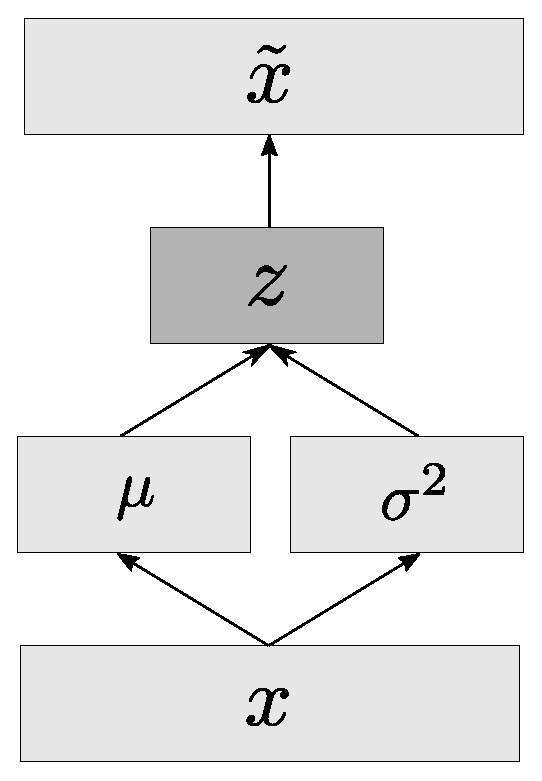
\includegraphics[scale=0.45]{background/variational_autoencoder_naive.eps}
\caption{A na\"{i}ve implementation of the variational autoencoder. The input $\vec{x}$ is mapped to intermediate layers taking the values of $\vec{\mu}$ and $\vec{\sigma}^2$. The latent variable $\vec{z}$ is then sampled from the probabilistic encoder $\vec{z} \sim q_{\vec{\phi}}(\vec{z} | \vec{x})$. Finally $\vec{z}$ is mapped back to the input dimension to give reconstruction $\vec{\tilde{x}}$.}
\label{fig:variational_autoencoder_naive}
\end{figure}

Unfortuntely we cannot perform backpropagation, as it makes no sense to differentiate the the random variable $\vec{z}$ wrt $\vec{\phi}$ ($\vec{z}$ is drawn from a distribution, and not a function of $\vec{\phi}$). To solve this, we introduce an auxillary variable $\vec{\epsilon}$ and vector-valued function $g_{\phi}(\vec{x}, \vec{\epsilon})$ parameterised by $\vec{\phi}$ \cite{Kingma2014}. The auxillary variable $\vec{\epsilon}$ is governed by a parameterless distribution, which we will take to be the multivariate isotropic Gaussian.

The sampling step can now be written as
\begin{align}
\vec{z} = g_{\vec{\phi}}(\vec{x}, \vec{\epsilon}) = \vec{\mu} + \vec{\sigma} \odot \vec{\epsilon} \quad\quad\quad \vec{\epsilon} \sim \mathcal{N}(\vec{0}, \vec{I})
\end{align}
where $\odot$ represents the element-wise product. This is a reparameterisation of the random variable $\vec{z}\sim q_{\vec{\phi}}(\vec{z}|\vec{x})$ with a differentiable function $g_{\vec{\phi}}(\vec{x}, \vec{\epsilon})$, and is suitable known as the ``reparameterisation trick" \cite{Kingma2014}. The reparameterisation trick allows backpropagation to be used, and thus completes our method of solving optimisation problem (\ref{eq:elbo_optimisation_problem}).\\

\begin{figure}[h!]
\centering
\captionsetup{justification=centering}
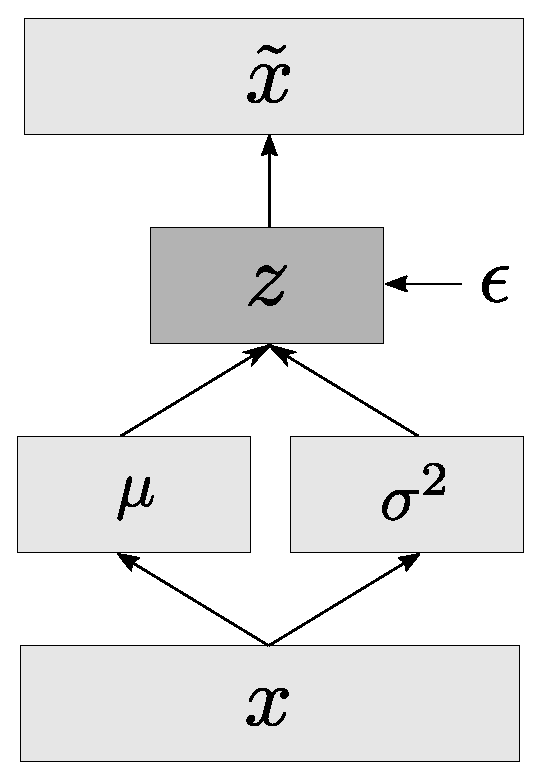
\includegraphics[scale=0.45]{background/variational_autoencoder_reparameterisation_trick.eps}
\caption{A viable implementation of the variational autoencoder. Sampling from the probabilistic encoder $q_{\vec{\phi}}(\vec{z} | \vec{x})$ is simulated by evaluating $\vec{z} = g_{\vec{\phi}}(\vec{x}, \vec{\epsilon}) = \vec{\mu} + \vec{\sigma} \odot \vec{\epsilon}$.}
\label{fig:variational_autoencoder_reparameterisation_trick}
\end{figure}

\newpage
\subsection{Intuition Behind the Variational Autoencoder}
In this section, we'll develop the intuition behind the variational autoencoder. We've been considering the data set $X = \{ \vec{x}^{(i)} \}_{i=1}^{N}$. Now we'll choose $X$ to be the MNIST data set (the vector $\vec{x^{(i)}}$ now corresponds to a flattened MNIST image of length $28\times 28 = 784$). For visualisation purposes, we'll also take the latent space dimension to be $k = 2$, that is, $\vec{z} = (z_1, z_2)$.

The probabilistic encoder
\begin{align}
q_{\vec{\phi}}(\vec{z} | \vec{x}^{(i)}) = \mathcal{N}(\vec{\mu}^{(i)}, \vec{\sigma}^{2(i)}\vec{I})
\tag{\ref{eq:approximate_posterior_gaussian}}
\end{align}

gives a normal distribution over the values of the latent variable $\vec{z}^{(i)}$ given data point $\vec{x}^{(i)}$. A sample is drawn from this normal distribution and passed through to the decoder. The decoder then reconstructs the original image from the latent representation. Since we've chosen our latent space to be two-dimensional, it's possible to visualise this process, which is done in Figure (\ref{fig:variational_autoencoder_latent_space_colour_0_with_mnist_updated}). It's then possible to compare the reconstruction to the original (using an appropriate reconstruction loss function), and therefore to train the autoencoder as a whole.

Recall that we chose the prior to be the standard multivariate Gaussian
\begin{align}
p_{\vec{\theta}}(\vec{z}) = \mathcal{N}(\vec{0}, \vec{I})
\tag{\ref{eq:variational_autoencoder_prior_standard_gaussian}}
\end{align}
We also derived the loss function to be
\begin{align}
\mathcal{L}(\vec{\theta}, \vec{\phi}; \vec{x}^{(i)}) = -D_{KL}(q_{\vec{\phi}}(\vec{z}|\vec{x}^{(i)}) || p_{\vec{\theta}}(\vec{z})) + \mathbf{E}_{q_{\vec{\phi}}(\vec{z}|\vec{x}^{(i)})}\big[\log p_{\vec{\theta}}(\vec{x}^{(i)} | \vec{z}) \big]
\tag{\ref{eq:elbo_kl_loss_plus_expectation}}
\end{align}
which we want to maximise. Since
\begin{align}
D_{KL}(q_{\vec{\phi}}(\vec{z}|\vec{x}^{(i)}) || p_{\vec{\theta}}(\vec{z})) \geq 0
\end{align}
maximising the $ELBO$ is eqiuvalent to ruducing the KL divergence between the probabilistic encoder $q_{\vec{\phi}}(\vec{z}|\vec{x}^{(i)})$ and the prior $p_{\vec{\theta}}(\vec{z})$. Therefore after training, we expect that the probabilistic encoder should map samples to the standard multivariate Gaussian. (In practice, $\mathcal{L}(\vec{\theta}, \vec{\phi}; \vec{x}^{(i)}) > 0 \quad \forall i$, so we therefore only expect it to be \textit{approximately} mapped to the standard Gaussian). Decoding samples from the prior should correspond to meaningful reconstructions.

TODO: FINISH

\begin{figure}[h!]
\centering
\captionsetup{justification=centering}
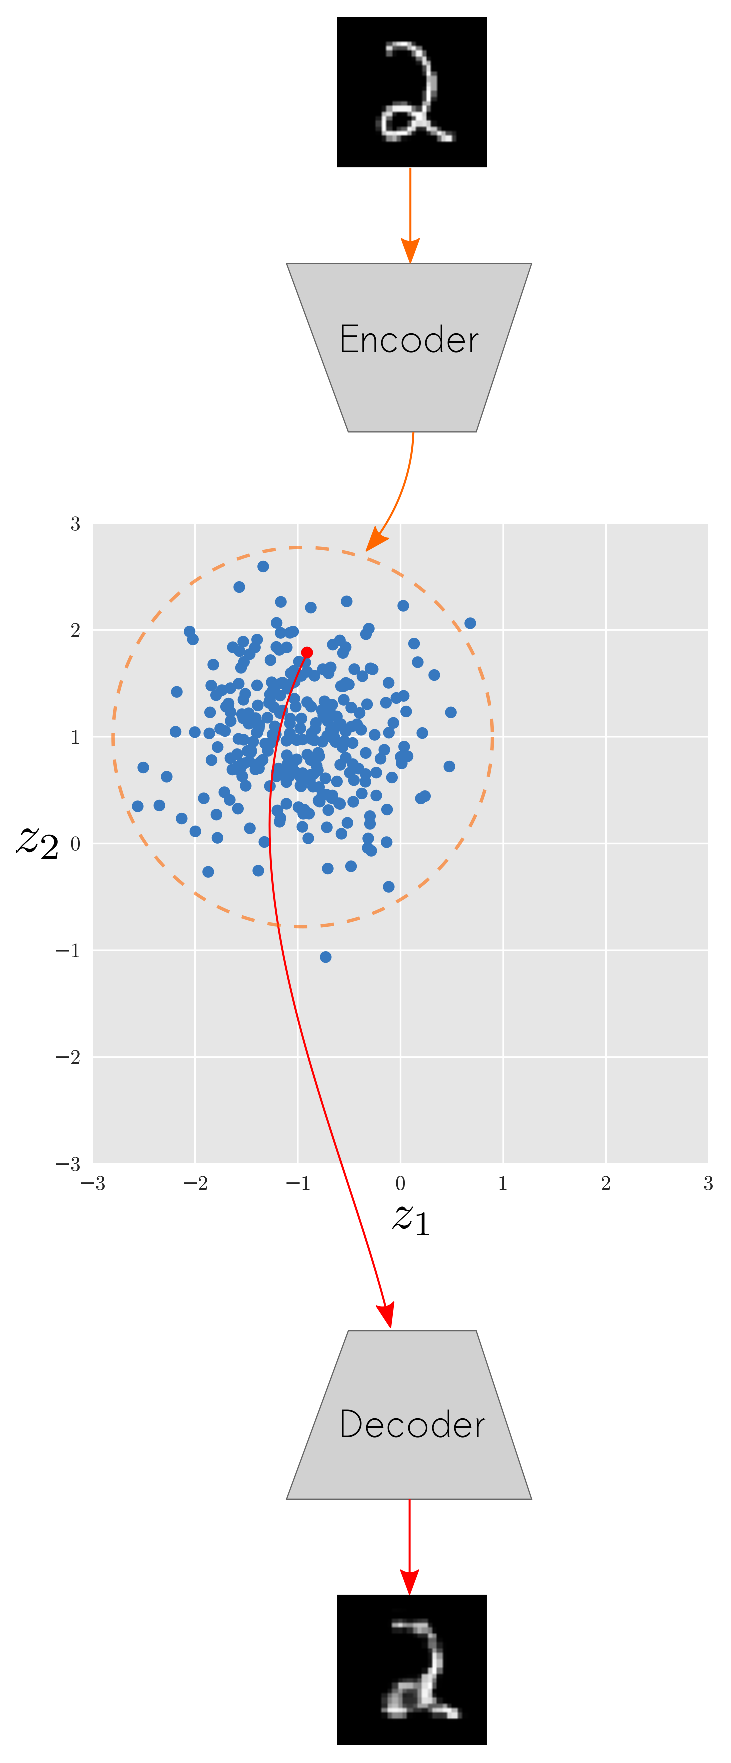
\includegraphics[scale=0.7]{background/variational_autoencoder_latent_space_colour_0_with_mnist_updated.eps}
\caption{The encoder takes a data point and returns a normal distribution (orange); some samples of which are shown (blue). A sample is drawn from the normal distribution (red) and decoded. \cite{Dykeman2016}}
\label{fig:variational_autoencoder_latent_space_colour_0_with_mnist_updated}
\end{figure}

\begin{figure}[h!]
\centering
\captionsetup{justification=centering}
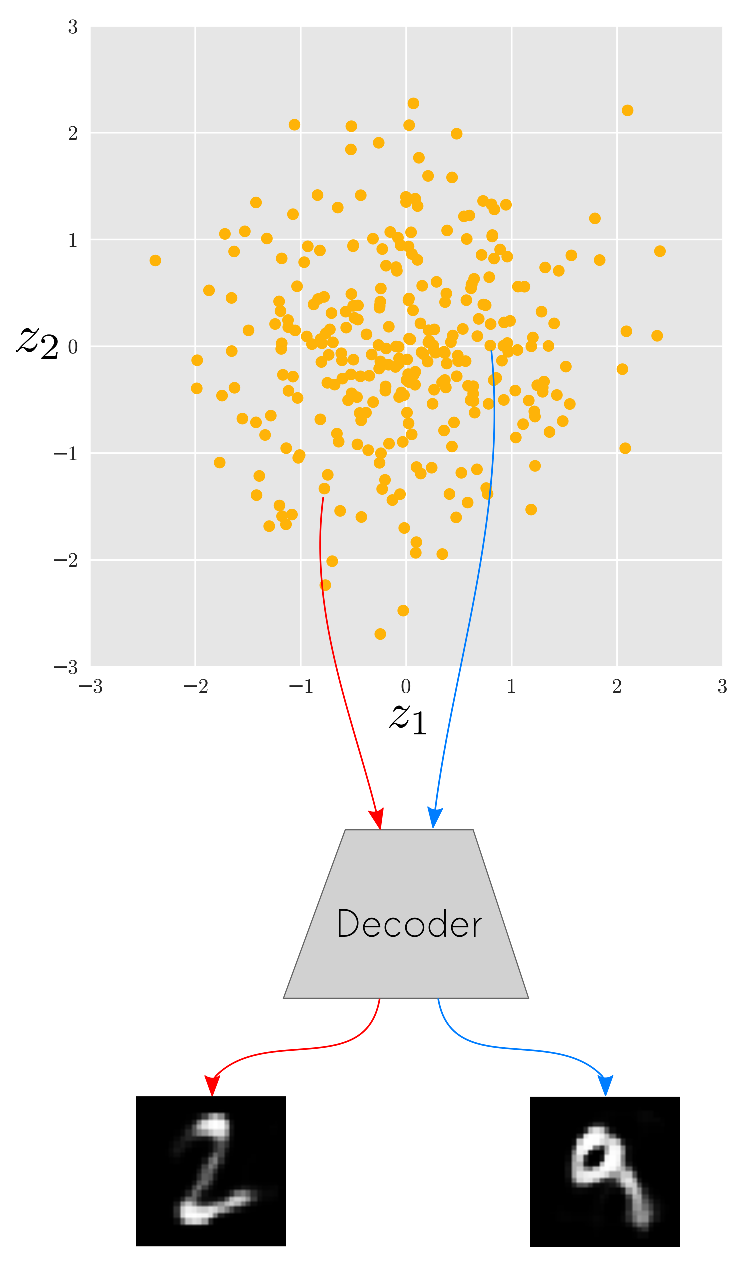
\includegraphics[scale=0.7]{background/variational_autoencoder_latent_space_unit_gaussian_with_mnist.eps}
\caption{The prior distribution should approximate the standard multivariate Gaussian $\mathcal{N}(\vec{0}, \vec{I})$. Samples of the prior are shown (yellow); two of which are decoded (red and blue). \cite{Dykeman2016}}
\label{fig:variational_autoencoder_latent_space_unit_gaussian_with_mnist}
\end{figure}

\begin{landscape}
\begin{figure}[h!]
\centering
\captionsetup{justification=centering}
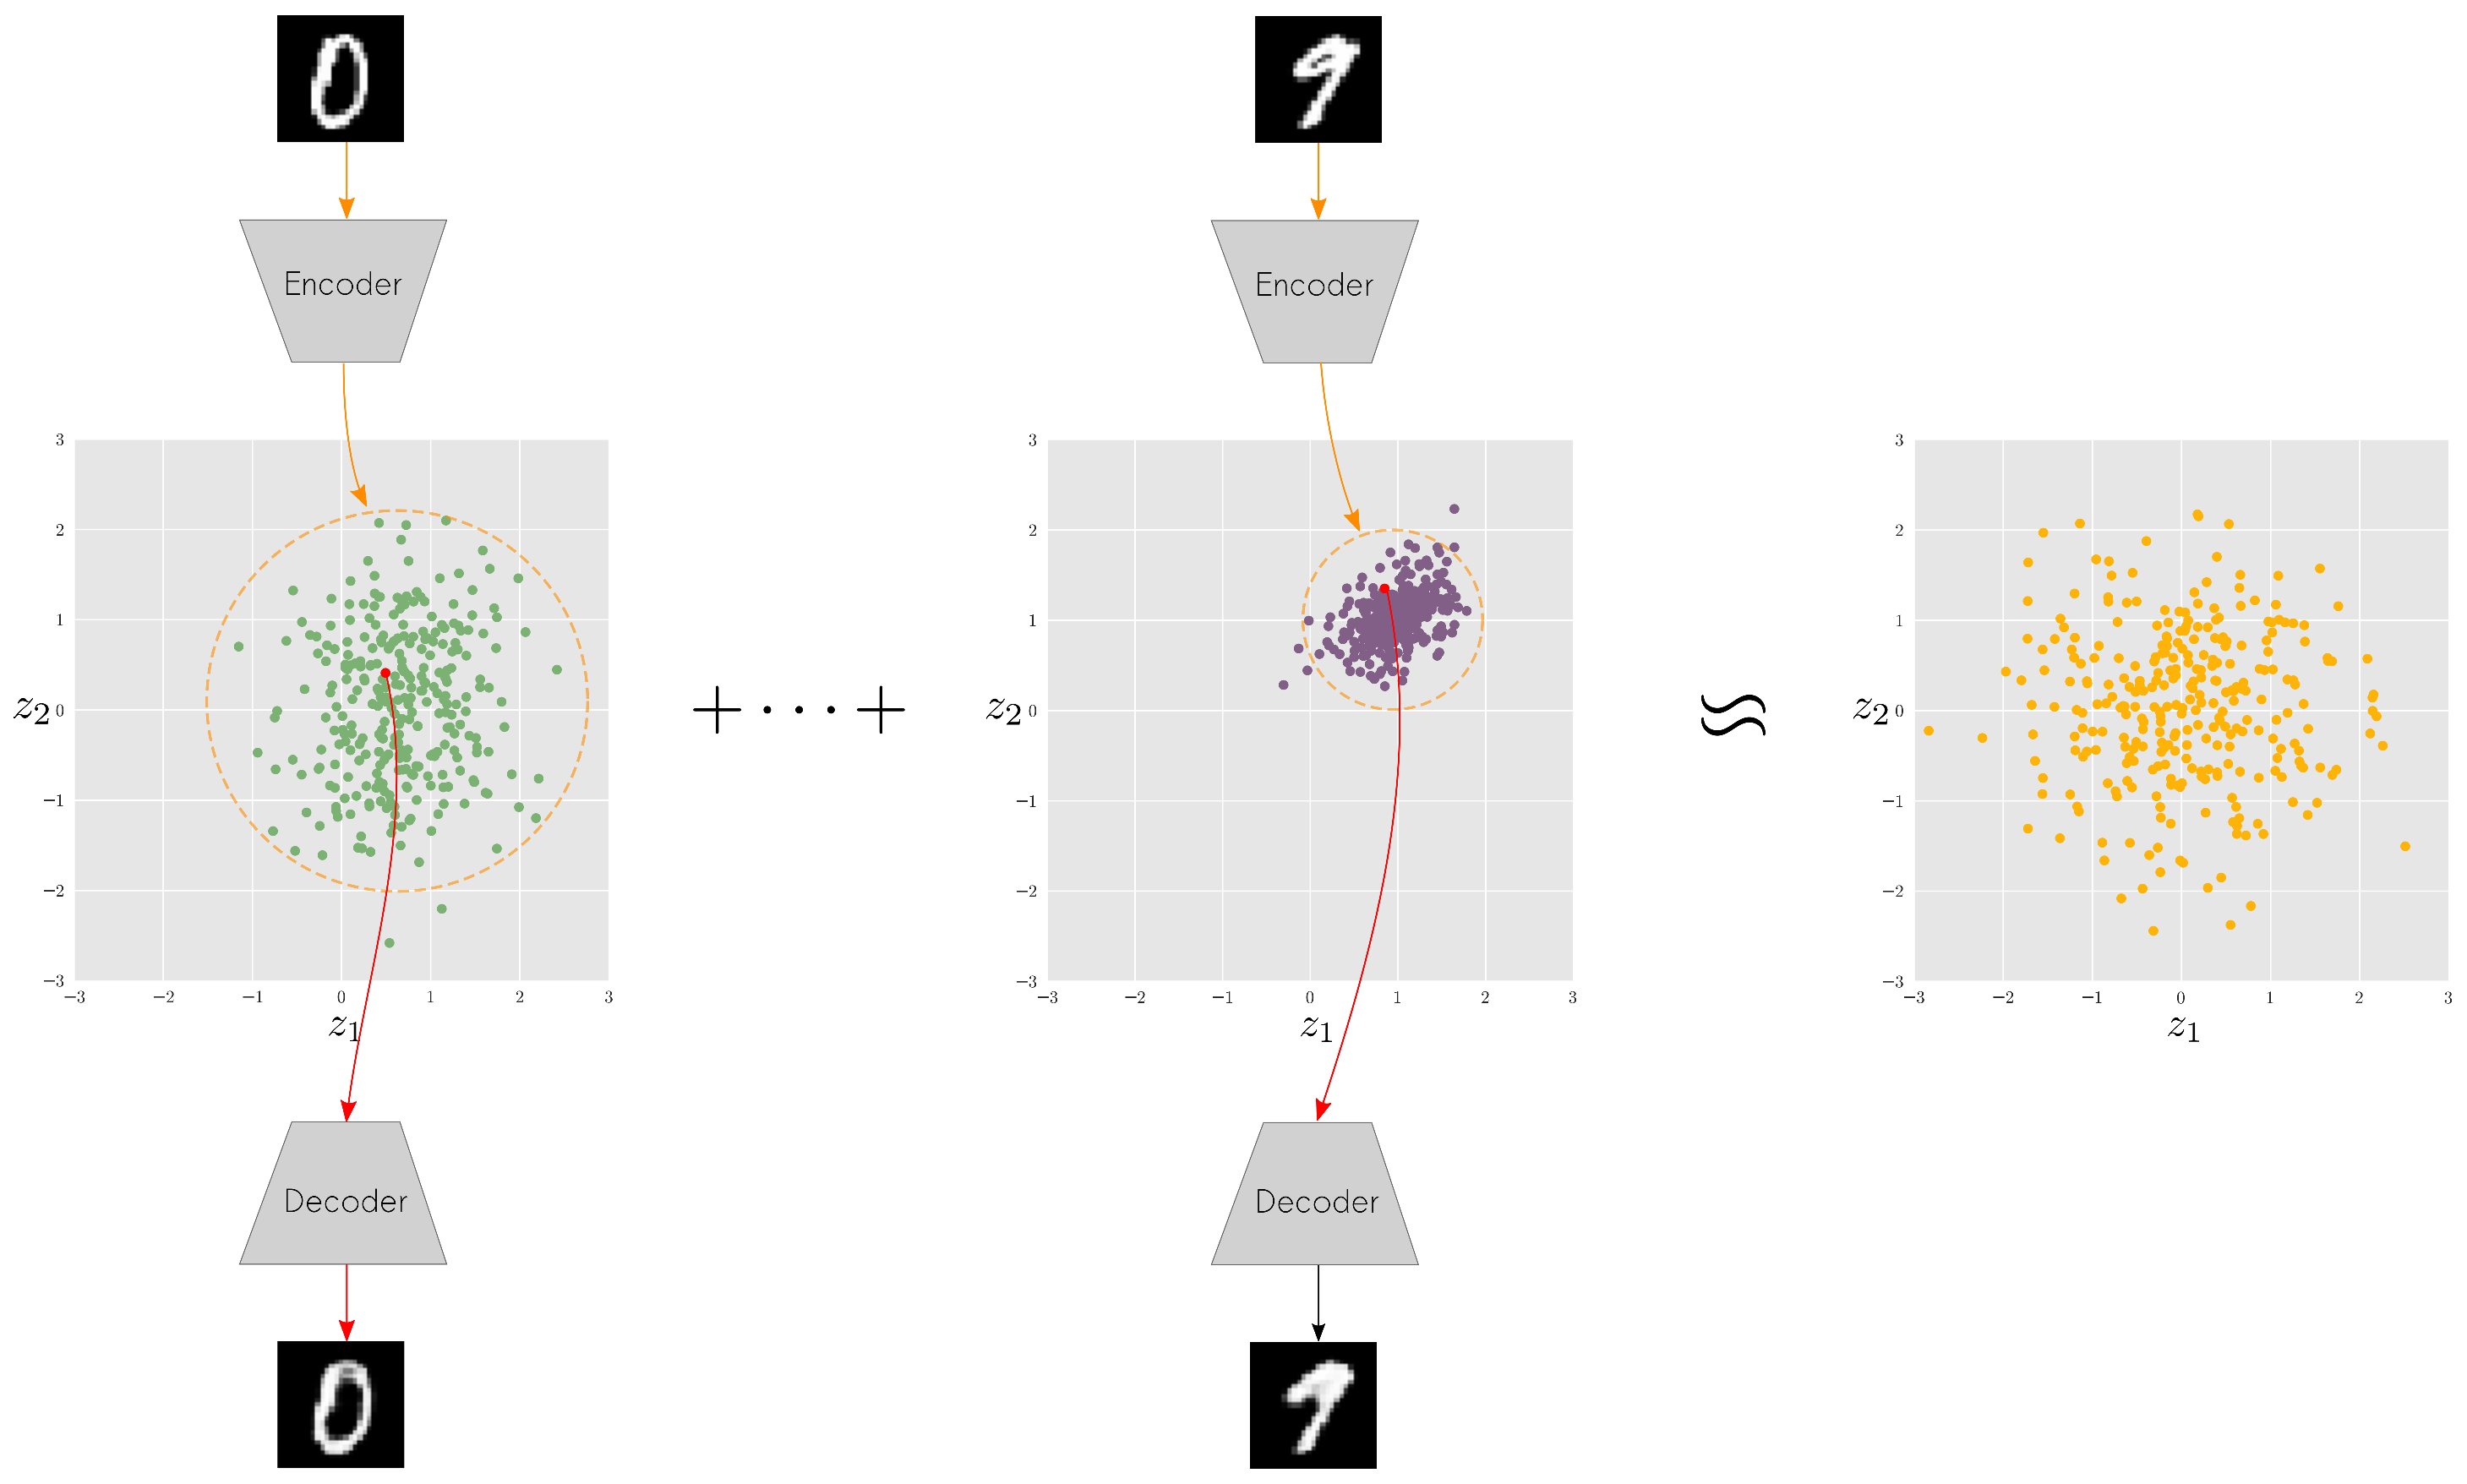
\includegraphics[scale=0.45]{background/variational_autoencoder_latent_space_adding_latent_spaces_updated.eps}
\caption{The sum over the latent space distributions of all data points $\vec{x}^{(i)}$ approximates the multivariate isotropic Gaussian. \cite{Dykeman2016}}
\label{fig:variational_autoencoder_latent_space_adding_latent_spaces_updated}
\end{figure}
\end{landscape}



%
%
%
%
%
\section{Disentangled Representations}
\cite{Higgins2016, Thiagarajan2016}





%
%
%
%
%
\section{Unsupervised Learning of Generative Factors}
Learning disentangled generative factors of a scene in an unsupervised manner is an open challenge in AI research. Although many attempts have been made, they have not scaled well \cite{Thiagarajan2016, Schmidhuber1992, Desjardins2012, Tang2013, Cohen2014}. However, two recent advancements have made significant headway: $\beta$-VAE and InfoGAN \cite{Chen2016, Thiagarajan2016}.

\subsection{InfoGAN}
InfoGAN is an information theoretic extension of the Generative Adversarial Network, which has convincingly learnt generative factors of multiple data sets in an unsupervised manner, including MNIST, 3D faces and 3D chairs \cite{Chen2016}.

\begin{figure}[h!]
\centering
\captionsetup{justification=centering}
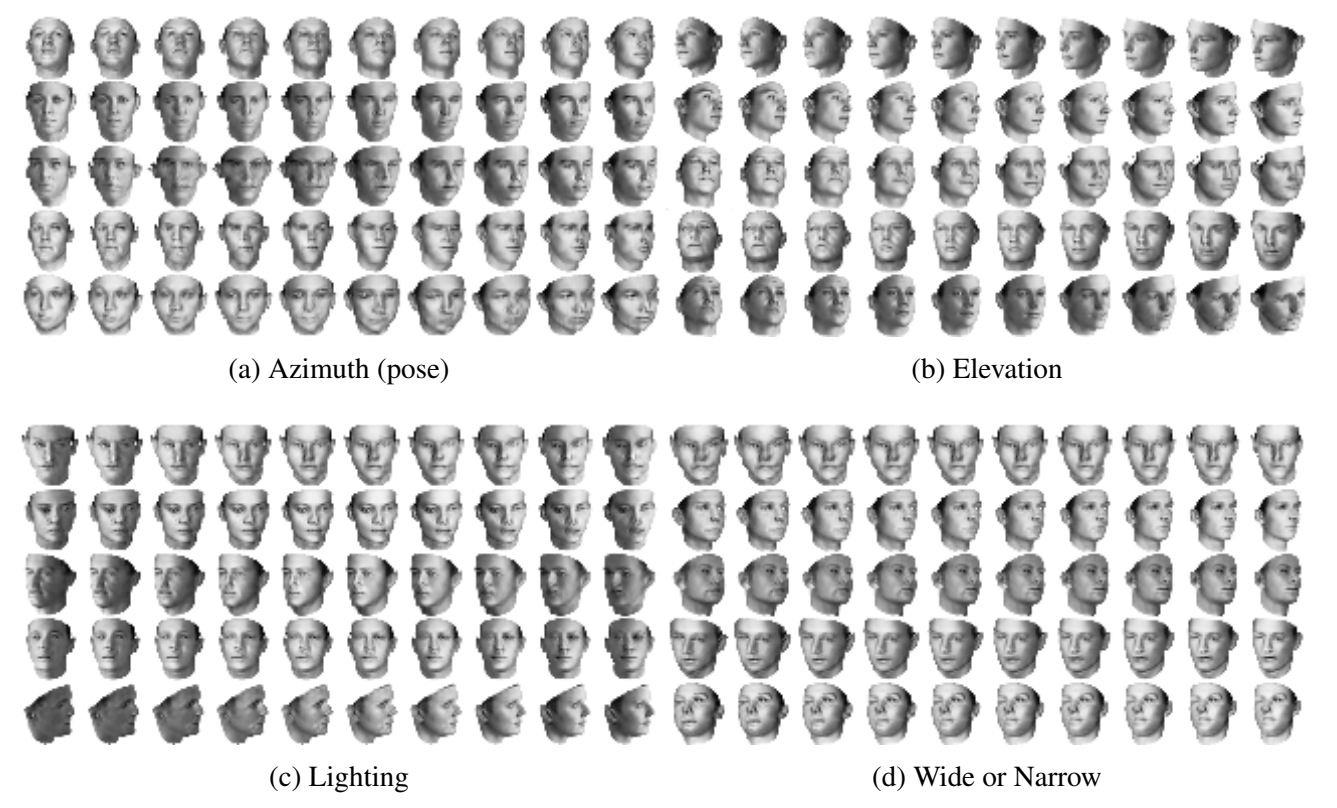
\includegraphics[scale=0.36]{related_work/info_gan_3d_face_dataset.png}
\caption{InfoGAN convincingly learns the underlying generative factors in the 3D face data set. Rows correspond to a data point and columns the value of the latent variable (varied from $-1$ to $1$). Each section (a), (b), (c) and (d) consider a different latent variable. \cite{Chen2016}}
\label{fig:info_gan_3d_face_dataset}
\end{figure}

However, InfoGAN is sensitive to the choice of the prior distribution, and therefore requires a priori knowledge of the data set, as well as the number and type of generative factors \cite{Thiagarajan2016}. Ideally, the number of generative factors would be inferred and not made explicit by the designer. On this basis, we can conclude that future work is needed.

\subsection{$\beta$-VAE}
$\beta$-VAE is the first method to overcome what InfoGAN could not: to learn the (unspecified amount of) generative factors of a data set in an unsupervised manner. First a formal derivation of $\beta$-VAE will be proposed, then a number of experimental results.

\subsubsection{Derivation}
Recall that for the variational autoencoder, we assumed the data point $\vec{x}$ was generated by a process involving a latent variable $\vec{z}$ and conditional $p(\vec{x}|\vec{z})$. For $\beta$-VAE we make a slightly different assumption: data point $\vec{x} \in \mathbb{R}^N$ was generated by conditionally independent factors $\vec{v} \in \mathbb{R}^K$ s.t. $p(\vec{v} | \vec{x}) = \prod_k p(v_k | \vec{x})$, conditionally dependent factors $\vec{w} \in \mathbb{R}^H$ and the conditional $p(\vec{x} | \vec{v}, \vec{w})$. In short, this is written as
\begin{align}
p(\vec{x}|\vec{v}, \vec{w}) = Sim(\vec{v}, \vec{w})
\end{align}
where $Sim$ is short for a true world simulator. $\beta$-VAE seeks to represent these generative factors in the latent variable $\vec{z} \in \mathbb{R}^M$, such that
\begin{align}
p(\vec{x} | \vec{z}) \approx p(\vec{x} | \vec{v}, \vec{w}) = Sim(\vec{v}, \vec{w})
\end{align}
Note that, unlike InfoGAN, $\beta$-VAE does not specify the number independent generative factors $K$; instead it is inferred. However, in order for $\vec{z} \in \mathbb{R}^M$ to learn the conditionally independent factors $\vec{v} \in \mathbb{R}^K$, we must assert that $M \geq K$.

As before, the posterior $p_{\vec{\theta}}(\vec{z}|\vec{x})$ is intractable, which motivates the introduction of the probabilistic encoder $q_{\vec{\phi}}(\vec{z} | \vec{x})$. A reasonable objective is to find the most likely parameters of the model over all latent variables that produced the observed data. This is summarised more precisely as the optimisation problem
\begin{align}
\vec{\theta}^*, \vec{\phi}^* = \max_{\vec{\phi}, \vec{\theta}} \mathbf{E}_{q_{\vec{\phi}}(\vec{z} | \vec{x})} \big[ \log p_{\vec{\theta}}(\vec{x} | \vec{z}) \big]
\end{align}
A constraint is added to control the capacity of information in the latent space and encourage the factors $\vec{v}$ to be learnt in a disentangled manner. The probabilistic encoder $q_{\vec{\phi}}(\vec{z} | \vec{x})$ is pressured to be close to an isotropic Gaussian, implicitly applying an independence pressure. By using the KL divergence, we form the optimisation problem
\begin{align}
\vec{\theta}^*, \vec{\phi}^* &= \max_{\vec{\phi}, \vec{\theta}} \mathbf{E}_{q_{\vec{\phi}}(\vec{z} | \vec{x})} \big[ \log p_{\vec{\theta}}(\vec{x} | \vec{z}) \big] \label{eq:beta_vae_optimisation_problem}\\
&\textup{s.t. } D_{KL} (q_{\vec{\phi}}(\vec{z} | \vec{x}) || p(\vec{z})) < \epsilon \nonumber
\end{align}
The Lagrangian of optimisation problem (\ref{eq:beta_vae_optimisation_problem}) is
\begin{align}
\mathcal{F}(\vec{\theta}, \vec{\phi}; \vec{x}) = \mathbf{E}_{q_{\vec{\phi}}(\vec{z} | \vec{x})} \big[ \log p_{\vec{\theta}}(\vec{x} | \vec{z}) \big] - \beta(D_{KL} (q_{\vec{\phi}}(\vec{z} | \vec{x}) || p(\vec{z})) - \epsilon)
\end{align}
Since $\beta, \epsilon > 0$,
\begin{align}
\mathcal{F}(\vec{\theta}, \vec{\phi}; \vec{x}) \geq \mathcal{L}(\vec{\theta}, \vec{\phi}; \vec{x}) = \mathbf{E}_{q_{\vec{\phi}}(\vec{z} | \vec{x})} \big[ \log p_{\vec{\theta}}(\vec{x} | \vec{z}) \big] - \beta D_{KL} q_{\vec{\phi}}(\vec{z} | \vec{x}) || p(\vec{z}))
\end{align}


By applying pressure for $q_{\vec{\phi}}(\vec{z} | \vec{x})$ to be close to the prior $p(\vec{z})$, the latent space learns the conditionally independent factors $\vec{v}$ in a different subset of $\vec{z}$ than the conditionally dependent factors $\vec{w}$. $\beta$ controls the degree of this pressure. Also note that $\beta = 1$ yields the $ELBO$ formulated earlier (\ref{eq:elbo_reconstruction_kl_divergence}), and $\beta=0$ yields the maximum likelihood case. It's hypothesised that disentangled representations are learnt for $\beta > 1$.

As the prior needs to be isotropic, it's often chosen to be the standard multivariate Gaussian:
\begin{align}
p(\vec{z}) = \mathcal{N}(\vec{0}, \vec{I})
\end{align}

\begin{figure}[h!]
\centering
\captionsetup{justification=centering}
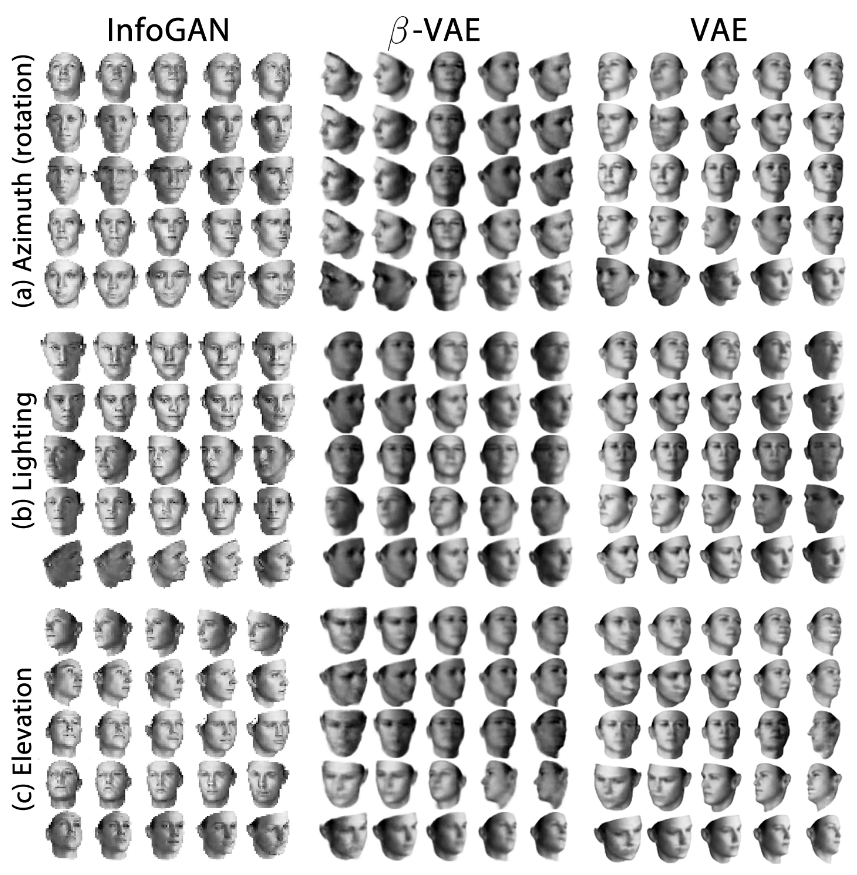
\includegraphics[scale=0.44]{related_work/beta_vae_3d_face_dataset_comparison.png}
\caption{A comparison of InfoGAN, $\beta$-VAE ($\beta = 20$) and VAE on the 3D face data set. Different latent variables are varied for sections (a), (b) and (c). All models learnt lighting and elevation, but only InfoGAN and $\beta$-VAE managed to continuously vary the azimuth. \cite{Thiagarajan2016}}
\label{fig:beta_vae_3d_face_dataset_comparison}
\end{figure}



%
%
%
%
%
\section{Improving Sampling from Generative Autoencoders with Markov Chains}

A generative autoencoder may be defined as an autoencoder that pressures its latent distribution $q_{\phi}(\vec{z} | \vec{x})$ to match a given prior $p(\vec{z})$ \cite{Creswell2016}. As discussed earlier, the KL divergence term in the $ELBO$ applies this pressure:
\begin{align}
\mathcal{L}(\vec{\theta}, \vec{\phi}; \vec{x}) = -D_{KL}(q_{\vec{\phi}}(\vec{z}|\vec{x}) || p_{\vec{\theta}}(\vec{z})) + \mathbf{E}_{q_{\vec{\phi}}(\vec{z}|\vec{x})}\big[\log p_{\vec{\theta}}(\vec{x} | \vec{z}) \big]
\tag{\ref{eq:elbo_kl_loss_plus_expectation}}
\end{align}

In Section (\ref{sec:variational_autoencoders}) it was assumed that the data set $X$ was generated by
\begin{align}
\vec{z}^{(i)} \sim p(\vec{z}) \quad\quad \vec{x}^{(i)} \sim p_{\vec{\theta}^*}(\vec{x} | \vec{z}^{(i)})
\end{align}
where $p(\vec{z})$ is a parameterless prior distribution and $p_{\vec{\theta}^*}(\vec{x} | \vec{z}^{(i)})$ is the true conditional. As the true set of parameters $\vec{\theta}^*$ is unknown to us, we may attempt to generate samples with learnt parameters $\vec{\theta}$:
\begin{align}
\vec{z}^{(i)} \sim p(\vec{z}) \quad\quad \vec{x}^{(i)} \sim p_{\vec{\theta}}(\vec{x} | \vec{z}^{(i)})
\label{eq:sampling_procedure_naive}
\end{align}
Now suppose
\begin{align}
\int q_{\vec{\phi}}(\vec{z} | \vec{x}) p(\vec{x})d\vec{x} = \hat{p}(\vec{z})
\end{align}
where $p(\vec{x})$ is the distribution that generated data set $X$. The generative procedure (\ref{eq:sampling_procedure_naive}) makes the erroneous assumption that $q_{\vec{\phi}}(\vec{z} | \vec{x})$ perfectly matches the prior $p(\vec{z})$, that is, $p(\vec{z}) = \hat{p}(\vec{z})$ \cite{Creswell2016}. Since only pressure was applied to match the two, this is clearly not true in general. That is, in general,
\begin{align}
p(\vec{z}) \neq \hat{p}(\vec{z})
\end{align}
Therefore we have
\begin{align}
\int p_{\vec{\theta}}(\vec{x | \vec{z}}) \hat{p}(\vec{z}) d\vec{z} = p(\vec{x}) \neq \int p_{\vec{\theta}}(\vec{x | \vec{z}}) p(\vec{z}) d\vec{z}
\end{align}
which suggests that the generative procedure (\ref{eq:sampling_procedure_naive}) does not produce samples from $p(\vec{x})$ exactly. To sample from $p(\vec{x})$, a new generative procedure is proposed \cite{Creswell2016}:
\begin{align}
\vec{z}^{(i)} \sim \hat{p}(\vec{z}) \quad\quad \vec{x}^{(i)} \sim p_{\vec{\theta}}(\vec{x} | \vec{z}^{(i)})
\label{eq:updated_sampling_mcmc}
\end{align}

\begin{figure}[h!]
\centering
\captionsetup{justification=centering}
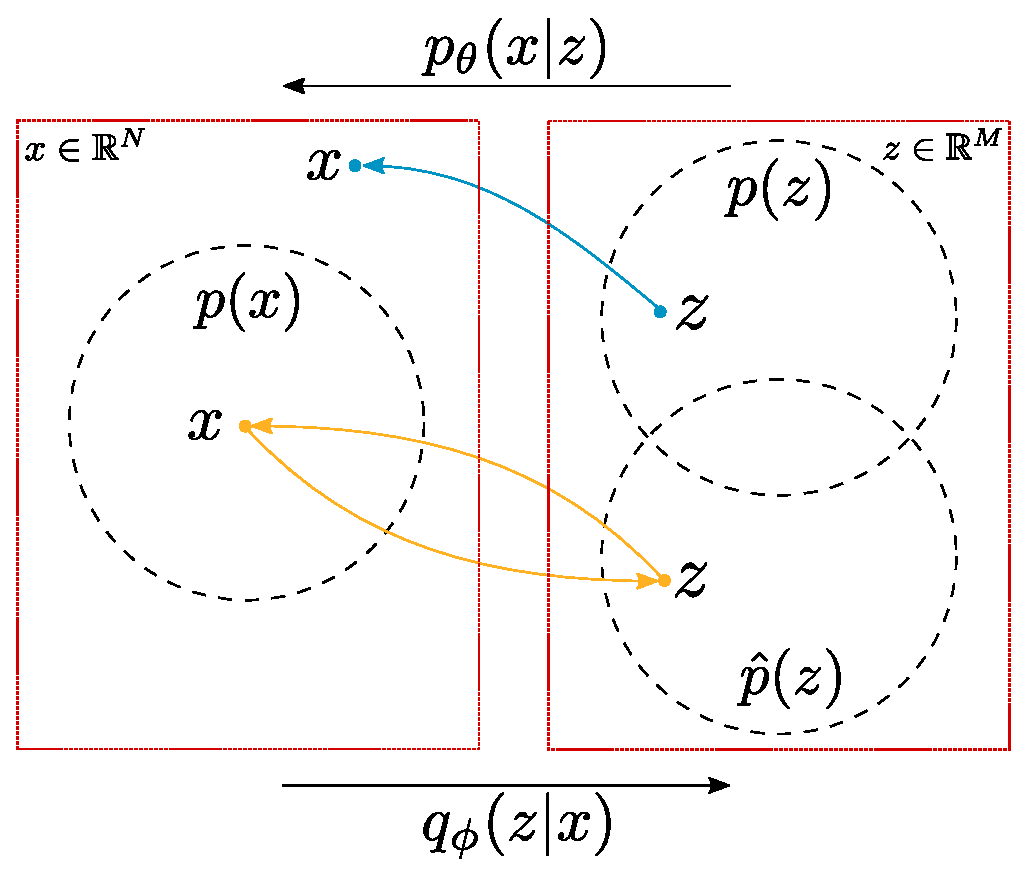
\includegraphics[scale=0.6]{related_work/mcmc_sampling.eps}
\caption{The probabilistic encoder $q_{\vec{\phi}}(\vec{z} | \vec{x})$ maps a given data point $\vec{x}$ to the unknown distribution $\hat{p}(\vec{z})$. The probabilistic decoder $p_{\vec{\theta}}(\vec{x} | \vec{z})$ is trained to map samples from $\hat{p}(\vec{z})$ back to $p(\vec{x})$, since its inputs are drawn from the probabilistic encoder $q_{\vec{\phi}}(\vec{z} | \vec{x})$. A sample from the prior $p(\vec{z})$ will not be mapped back by $p_{\vec{\theta}}(\vec{x} | \vec{z})$ to $p(\vec{x})$ exactly if $p(\vec{z}) \neq \hat{p}(\vec{z})$. \cite{Creswell2016}}
\label{fig:mcmc_sampling}
\end{figure}

As $\hat{p}(\vec{z})$ is unknown, it is not obvious how to sample from generative autoencoders using procedure (\ref{eq:updated_sampling_mcmc}). However, it is possible to formulate a Markov chain Monte Carlo (MCMC) chain that starts with an arbitrary latent variable $\vec{z}_{t=0}$ and converges with $\vec{z}_{t \rightarrow \infty} \sim \hat{p}(\vec{z})$ \cite{Creswell2016}. This is done by successively encoding and decoding the same sample as follows:
\begin{align}
\vec{x}_{t=k+1} \sim p_{\vec{\theta}}(\vec{x} | \vec{z}_{t=k}) \quad\quad \vec{z}_{t=k+1} \sim q_{\vec{\phi}}(\vec{z} | \vec{x}_{t=k+1})
\label{eq:mcmc_sampling}
\end{align}
where $\vec{z}_{t=0}$ is arbitrarily chosen.

\begin{figure}[H]
\centering
\captionsetup{justification=centering}
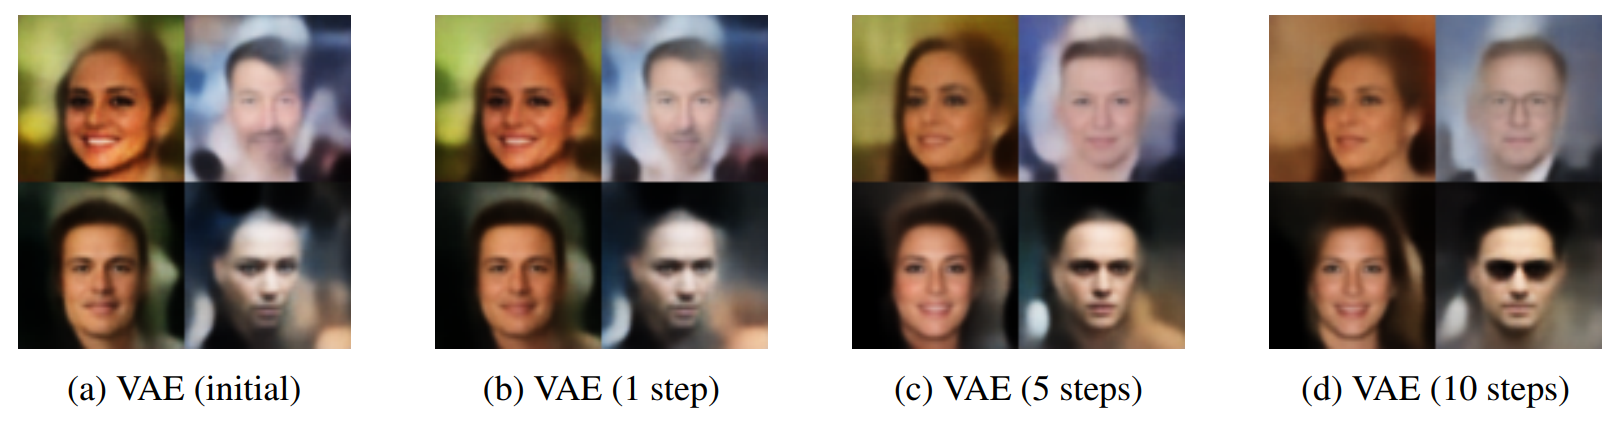
\includegraphics[scale=0.30]{related_work/celeb_a_vae_mcmc.png}
\caption{Samples from a variational autoencoder trained on the CelebA data set after $t = 0, 1, 5$ and $10$ steps of the generative procedure (\ref{eq:mcmc_sampling}). The MCMC chain was initialised with a sample from the prior $\vec{z}_{t=0} \sim p(\vec{z})$, which often improves the quality of the samples. \cite{Creswell2016}}
\label{fig:mcmc_sampling}
\end{figure}



%
%
%
%
%
\section{Regularizing CNNs with Locally Constrained Decorrelations}
\cite{Rodriguez2016}




%
%
%
%
%
\section{Batch Normalisation}
...